% !TeX root = ./1-handout.tex

%details on counters; setting it to 0 prints everything with a roman I
%https://www.overleaf.com/learn/latex/Counters

%https://tex.stackexchange.com/questions/555149/how-do-i-change-the-frame-continuation-counter-from-roman-numerals-i-ii-iii

% They could incorporate/do if needing to kill time:
% chalk and talk the review sheet for this week
% talk about the strangeness of reductio proofs (could do this in future as well!); but defs relevant this week given large number of reductio proofs on the pset 
%changes to notion of rigor in mathematics; e.g. bolzano moving away from physical intuition , motion, passage of time. 

% One possibly fun thing to talk through as a philosophy prompt: the definition of the function was initially contested. Some people thought that functions must be continuous. Get some more examples. In what sense, if any, should we believe that our definition of `function' is the canonical or correct one? To what extent, if any, should we think that the notion of `function' is a human construct? (Discovery vs. invention)

%\newcounter{mysection}
%\setcounter{mysection}{1}
%\arabic{mysection}
%\roman{subsection}

%\begin{itemize}[<+->] 
%\item<2-> % reveals second and keeps on page in subsequent frames
%\begin{itemize}[<2->] %does for a whole list of items


\setcounter{section}{0} %sets section counter to 0. note that need to switch section counter from Roman to arabic for this to work! since no roman numeral for 0! %put this into preamble, i.e. file common.tex: \renewcommand\thesection{\arabic{section}}




\section{Infinite Cardinalities!}
%\subsection*{test}

\begin{frame}
%\large

\scriptsize{\tableofcontents}

\end{frame}


\begin{frame}
\frametitle{Things Hunt remains liable to forget to mention}
%\large

\begin{itemize}[<+->]


\item If you are on the waitlist and in class today, please let Hunt know after class and write your email (legibly) 

\item Feel free to join \href{https://piazza.com/mit/spring2023/24118}{Piazza}! 

\item Feel free to join PSet partners!!! 
\item[] Groups will be auto-assigned Tuesday (today?)

\item If you haven't yet, please complete the Most Basic Factz survey on Canvas
\item[] Attendance for last Tuesday 2/7/23

\item In light of a reading group beloved by Hunt, his Thursday OHs will now probably be 12--12:55 \& 3:45--4:40. 

\item If you're worried about legibility of your handwriting, send a sample to your TA or typeset your PSets! 



\end{itemize}
\end{frame}




 % \iffalse %*****************************************************

%\subsection{Time to get Injected!}
\subsection{Onto Injections! (They go both ways)}

\begin{frame}
\frametitle{Basics of Functions}
%\large

\begin{itemize}[<+->]

\item Consider a function $f$ (a.k.a. `map') from a \emph{domain} set $A$ to a \emphz{range} set $B$. We denote this as ``$f: A \rightarrow B$". 

\item To be \emph{well-defined}, EVERY element of $A$ must be mapped by $f$ to exactly one (not necessarily distinct) element of $B$

\item[] $\forall a \in A, \exists ! b \in B$ such that $f(a) = b$

\item[] (Note that the order of the quantifier matters a great deal: $\exists ! b \in B$ s.t. $\forall a \in A$,  $f(a) = b$ is a horizontal line if $A = B = \mathbb{R}$)

\item Note that the \emph{image} of $f$, ``$f(A)$", need not equal the entire range $B$: in general, $f(A) \subseteq B$

\item When the image equals $B$, we say that the function is \emph{onto}, a.k.a. ``a \emph{surjection}": $\forall b \in B, \exists a \in A$ s.t. $f(a) = b$

\end{itemize}
\end{frame}

\begin{frame}
\frametitle{Something we are all liable to forget to do!}
%\large

\begin{itemize}[<+->]

\item If you are asked to prove something that involves constructing a function $f: A \rightarrow B$, you ought to first show that the function is \emph{well-defined}:

\item i.e. that each element of the domain is sent to a unique element of the range

\item Is $f(x) = x^2$ where $f: \mathbb{R} \rightarrow \mathbb{N}$ well-defined? 
%no! e.g. 1/2 squared is 1/4 which is not in Naturals 

\item Basically, given an arbitrary $a \in A$, argue (i) that $f(a) \in B$ and that (ii) if there are $b \neq b'$ in $B$ such that both $b = f(a)$ and $b' = f(a)$ then we have a contradiction. 

\item Often, it is so seemingly `obvious' that a function is well-defined, that explicitly proving this will seem tedious and annoying.

\item[] \textit{spoiler}: philosophers have a tendency to be tedious ;) 

%\item Note that every element in the domain is sent to a single element in the range

% Note that the motivation for requiring functions to be well-defined is actually kind of interesting. You need different representatives of the same number to be sent to the same value, e.g. f(0.5) to equal f(1/2) and f(1) to equal f(0.9999999999) 


\end{itemize}
\end{frame}

\begin{frame}
\frametitle{Injections (ivermectin anyone?)}
%\large

\begin{itemize}[<+->]

\item \emph{Injection}: $\forall x, y \in A$, if $f(x) = f(y)$, then $x = y$.
\item[] Equivalently: $\forall x, y \in A$, if $x \neq y$, then $f(x) \neq f(y)$
%\item[] Intuitive gloss: each element $a$ of the domain $A$ is mapped to a unique element $b$ of the range $B$. 
\item[] If $a$ is mapped to $b$, then NO OTHER $x \in A$ is mapped to $b$
\item[] --Monogamous heterosexual norm-core marriages define an injection from monogamous-married men to women. 

\item  \emph{How to prove a function is injective}: consider two \textit{arbitrary} elements $x, y \in A$. Assume for the sake of argument that $f(x) = f(y)$. Proceed to show that $x=y$ (e.g. via algebra).

\item \emphz{How to prove a function is NOT injective}: \\ provide a concrete counterexample. i.e. identify two $x, y \in A$ such that $f(x) = f(y)$ but $x \neq y$.
\item[] e.g. $f(x) = x^4$, $f: \mathbb{Q} \rightarrow \mathbb{R}^{\geq 0}$

\end{itemize}
\end{frame}

\begin{frame}
\frametitle{Some Practice with Injections \& Surjections}
%\large

\begin{itemize}[<+->]

\item For each function below, determine whether it is (a) injective and (b) surjective:

\item Recall: Natural numbers $\mathbb{N} := \{ \mathbf{0}, 1, 2, \dots \}$ (we include zero!)

\item Integers $\mathbb{Z} := \{ \dots, -2, -1, 0, 1, 2, \dots \}$

\end{itemize}

\begin{enumerate}[<+->]

\item $f(x) = x+1$ where $f: \mathbb{N} \rightarrow \mathbb{N}$
%injective but not surjective because no natural number hits zero 

\item $f(x) = x^2$ where $f: \{ 1, 2, 3, \dots, 10 \} \rightarrow \{ 1, 2, \dots, 100 \}$
%injection but not surjection. e.g. 2 is not the square of anything in the domain 

\item $f(x) = x^2$ where $f: \{ -5, -4, \dots, -1, 0, 1, 2, \dots, 5\} \rightarrow \{ 0, 1, 4, 9, 16, 25 \}$

\item $f(x) = x^3$ where $f: \mathbb{Z} \rightarrow \mathbb{R}$
%injective but NOT surjective, e.g. no integer hits $\sqrt{2}$ or $\pi$ 

\end{enumerate}
\end{frame}

\begin{frame}
\frametitle{Bijections: injective surjections! (``1-to-1 and onto")}
%\large

\begin{itemize}[<+->]

\item A function $f: A \rightarrow B$ is a \emph{bijection} just in case it is \\ both (i) injective and (ii) surjective

\item[] e.g. $f(x) = x$ from $\mathbb{R}$ to $\mathbb{R}$ is a bijection 

\item \emph{To prove a bijection}: \textit{method one}: construct it! 
\item[] Show that the purported bijection $f$ is (0) well-defined, \\ (i) injective, and (ii) surjective

\item \emphz{Method Two}: use the Cantor-Schroeder-Bernstein Theorem:
\item[] (i) Construct an explicit injection in one direction, \\ then (ii) an injection in the other direction
\item[] -- Remember that injections don't have to be onto, so this can simplify things (e.g. if $A \subset B$, you can use the identity function)

\item \textbf{Method Three}: rely on known facts about \textit{cardinality} 


\end{itemize}
\end{frame}

\begin{frame}
\frametitle{On the History of ``Function"}
%\large

\begin{itemize}[<+->]

\item Our concept of ``function" developed over centuries

\item Dependence of one quantity on another in laws of nature, curves in Cartesian geometry, derivatives in calculus, analysis 

\item In the 19th century, definitions disagreed about whether functions have to be continuous
% e.g. Dirichlet's everywhere discontinuous function: define f(x) as 0 if x is rational and 1 if x is irrational 
%whereas Lobachevsky defined function in a way that required them to be continuous 
%Weierstrass's example of a continuous function which is nowhere differentiable 

\end{itemize}
\pause
\begin{quote}
\small{Poincar{\'e} in 1899: For half a century we have seen a mass of bizarre functions which appear to be forced to resemble as little as possible honest functions which serve some purpose. ... Formerly, when a new function was invented, it was in view of some practical end. Today they are invented on purpose to show that our ancestor's reasoning was at fault, and we shall never get anything more than that out of them. If logic were the teacher's only guide, he would have to begin with the most general, that is to say, the most weird functions.}
\end{quote}

\end{frame}

\begin{frame}
\frametitle{Philosophy Prompt(s) \#2}
%\large

\begin{itemize}[<+->]

\item How should we think about the evolution of the concept ``function" over centuries?

\item Should we think that mathematicians were refining their grip on a concept that in some sense \textit{always could have been defined} \\ (e.g. by the Babylonians, 1830–1531 BCE)?
%could do squares and cubes, and those are functions! written out in table form
%https://en.wikipedia.org/wiki/Babylonian_mathematics

\item In what sense, if any, is our concept of ``function" \textit{canonical} or \textit{privileged}?

\item Should we think that our concept is simply one of many that could be fruitful or interesting to focus on?

%e.g. maybe we should be focused on notion of morphism (generalization of homomorphism)in category theory. functions between sets are a special case of a morphism. 
%should we think that in math, a generalization is always more fundamental or to be privliged? what if a generalization is sterile? 


\end{itemize}
\end{frame}

\begin{frame}
\frametitle{Cardinality}
%\large

\begin{itemize}[<+->]

\item \emph{Cardinality}: shorthand for keeping track of the existence of bijections between sets

\item ``Two sets have the same cardinality" means: there exists a bijection between these two sets. 

\item $|A| = |B|$ if and only if $\exists$ bijection $f: A \rightarrow B$

\item We will discuss in what sense, if any, cardinality ought to be interpreted as the ``size" of a set. 

\end{itemize}
\end{frame}

\begin{frame}
\frametitle{Some practice with Bijections}
%\large

Recall: a bijection is an injective surjection 

\begin{enumerate}[<+->]

\item Construct a bijection from the integers to the natural numbers, $f: \mathbb{Z} \rightarrow \mathbb{N}$ (helps with a PSet \#1 problem)
% send the positive integers to the evens: 2n; send the negative integers to the odds: -2n -1

\item Construct a bijection from $\mathbb{N}$ to the set of prime numbers \\ (you may assume that given a finite set of primes, there is a \textit{smallest} prime number greater than every prime in that set)
%2022 Pset 1, number 7b; which I am changing to construct injection from set of integers to set of prime numbers. 


%\item Now a homework question! Construct a bijection from the set of integers to the set of prime numbers

%\item Construct a bijection from the set of prime numbers to the set of integers 

\end{enumerate}
\end{frame}


\begin{frame}
\frametitle{Some practice with Cardinality}
%\large
Between which of the following sets is it possible to construct a bijection (i.e. which sets have the same cardinality)?

\begin{enumerate}[<+->]

\item $\mathbb{Q}$ and the reals between 0 and 1, i.e. the interval $(0, 1)$ ?

\item $\mathbb{R}$ and $\mathscr{P}(\mathbb{N})$ ? 

\item $\mathbb{R}$ and $\mathscr{P}(\mathbb{R})$ ? 



\end{enumerate}

\end{frame}





%\iffalse %************************************************************************


\subsection{Puzzles about `Size'}
%could call this size-matters 

% % Josh read the following one**********************************************************
%https://en.wikipedia.org/wiki/Controversy_over_Cantor%27s_theory

\begin{frame}
%\frametitle{Stances: Vindication, Restriction, Revision}
\frametitle{To Vindicate, Restrict, or Revise/Reject?}
%\large

\begin{itemize}[<+->]

\item What attitude ought we take toward (parts of) math?
%\textit{what say you} about mathematics?

\item \emph{Vindication}: realism, formalism, structuralism, others

\item \emph{Meh}: error theory, quietism

\item \emph{Restriction}: naturalism, constructivism, finitism \\ -- retreat to a proper subset of math

\item \emph{Revision}: intuitionism, ultra-finitism
% Famous examples: folk psychology (churchlands); causation (russell)

\item Note that restriction and revision both involve \textit{rejecting} parts of classical math, to different extents. 

% Perhaps what is distinctive of revisionism is that it extends math in a way different from classical mathematics. Whereas the restriction accounts are a proper subset of classical math . But then perhaps I shouldn't call ultra-finitism a `revisionary' account?
% Maybe I can call ultra-finitism revisionary because it rejects even the finite part of classical math.

\item One true testament to the success of mathematics: \\ no one is trying to \emphz{eliminate} it, unlike other parts of our discourse 
%\item[] (e.g. folk psychology, causation, astrology, witchcraft \& wizardry)

%\item This is a continuum, so the divisions between `revision' and `rejection' can be a bit blurry. 


\end{itemize}
\end{frame}

\begin{frame}
  \frametitle{Happy Birthday to Fraenkel tm!}

  \begin{columns}
    \begin{column}{.5\textwidth}
      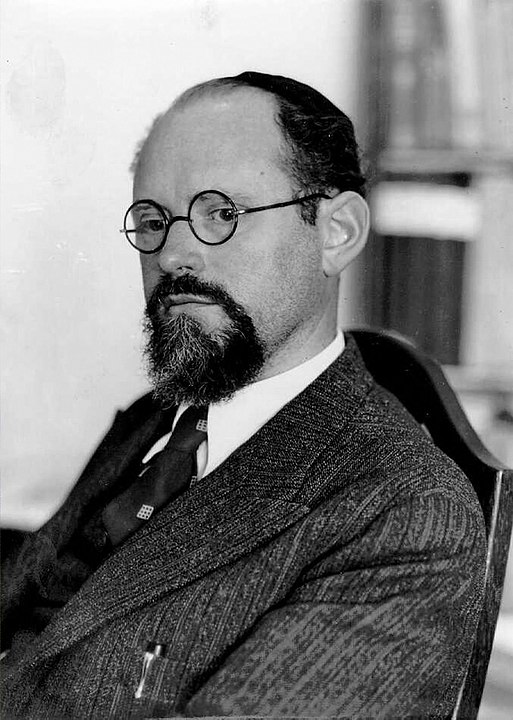
\includegraphics[height=.8\textheight]{../assets/Fraenkel_med}
    \end{column}
    \begin{column}{.5\textwidth}
      \begin{itemize}[<+->]
        \item Abraham Fraenkel (Feb 17th 1891--1965)
        \item One of the founders of Zermelo-Fraenkel set theory
\item Improved Zermelo's system in the 1920's. 
      \end{itemize}
    \end{column}
  \end{columns}
\end{frame}


\begin{frame}
\frametitle{Two Conceptions of `Size'}
%\large

\begin{itemize}[<+->]

\item \emphz{Proper Subset Principle}: if $A \subset B$, then B has more members than A. 
%logically, this is giving us a sufficient condition for difference in size 

\item[] e.g. $\mathbb{N} \subset \mathbb{Z}$ entails that there ``are more" integers than natural numbers (note: this is an apocryphal statement for the PSets!) 

\item \emph{Bijection Principle}: set $A$ has the same `size' as set $B$ if and only if there is a bijection from $A$ to $B$ 
%logically, this is giving necessary and sufficient conditions for same size. 
%so logically playing a different functional role than PSP, right from the start 

\item[] i.e. identify `size' with \textbf{cardinality} 

\item For many finite sets, these principles agree, but they disagree for infinite sets
% but they definitely don't agree for all finite sets, e.g. {0, 1, 2} vs. {3, 4, 5} have same size according to bijection principle but not according to proper subset principle! 
% Perhaps in the finite case, we can take bijection principle to be sufficient but not necessary for sameness of size. And proper subset principle is sufficient for difference in size?
% It does seem to be a problem that the proper subset principle cares about the identity of the elements, rather than just a more structural relationship

% % An improved proper subset principle? B has more members than A provided there exists sets C and D such that there is a bijection from B to D and A to C such that C is a proper subset of D

\end{itemize}
\end{frame}



\begin{frame}
\frametitle{Which Conception of Size should we Privilege?}
%\large

\begin{itemize}[<+->]

\item \emphz{Proper Subset Principle}:
\bi
\item accords better with our pre-theoretical intuitions

\item Intuitively, there are more rational numbers than natural numbers, since $\mathbb{N} \subset \mathbb{Q}$

\item Con: is mathematically sterile or `uninteresting' for infinite sets
% maybe one reason why proper subset principle is relatively uninteresting is that it is too restrictive to always have to focus on subsets. We want a more flexible notion, that allows for more isomorphisms between structures we could use for counting.

\ei

\item \emph{Bijection Principle}:
\bi

\item Is mathematically fruitful! 
%arguably b/c cardinality defines a total ordering on sets, so clear answers for size comparisons! 

\item Aside: what is fruitfulness in mathematics? \\ -- What does it mean for a bit of mathematics to be `interesting'?

\item Con: leads to some pretty crazy sounding claims, e.g. that the interval $[0, 1]$ has the same size as $\mathbb{R}$, even though clearly $[0,1]$ is a very small `part' of the interval $(-\infty, \infty)$

\ei

\end{itemize}
\end{frame}

\begin{frame}
\frametitle{An Improved Proper Subset Principle?}
%\large

\begin{itemize}[<+->]

\item What does the proper subset principle say about the relative size of $\{ 0, 1, 2 \}$ vs. $\{3, 4, 5 \}$? 

%What about $\{ 0, 1, 2 \}$ vs. $\{1, 2, 3, 4 \}$?

\item[] Not determined: neither set is a subset of the other 
%in both cases, neither set is a subset of the other 

\item What does the bijection principle say? 

\item[] BP saves intuition that these sets are the same size 
%and (ii) $\{1, 2, 3, 4 \}$ is bigger than $\{ 0, 1, 2 \}$
% I guess in the latter case, we are relying on something like the following: a set is bigger if there is an injection from the smaller set to the bigger set 

\end{itemize}
\end{frame}

\begin{frame}
\frametitle{Can we Modify the Proper Subset Principle?}
%\large

\begin{itemize}[<+->]

\item Goal: modify PSP such that the new rule gives the intuitive result for $\{ 0, 1, 2 \}$ vs. $\{3, 4, 5 \}$

\item \textbf{Better PSP(?)}: $B$ has more members than $A$ if and only if there exist sets $C$ and $D$ where (i) $C \subset D$ and (ii) there exist bijections from $B$ to $D$ and $A$ to $C$

\item Problem: contradictory results for infinite sets
\item[] e.g. let $A= B = \mathbb{N}$ and consider bijections $\mathbb{N} \rightarrow \mathbb{Z}$ and $\mathbb{N} \rightarrow \mathbb{N}$
%could we change into a necessary but not sufficient condition? 

\item Restrict to necessary condition? And take OG PSP as sufficient condition? 

\item Another option: restrict to finite sets 

%could we get into conflict here? e.g. have inconsistent size verdicts? 
%e.g. does this give result that N and Z have the same size? 

\end{itemize}
\end{frame}

\begin{frame}
\frametitle{Finitism: privilege subset principle}
%\large

\begin{itemize}[<+->]

\item Weyl against Cantor's set theory:

\begin{quote}
classical logic was abstracted from the mathematics of finite sets and their subsets.\dots Forgetful of this limited origin, one afterwards mistook that logic for something above and prior to all mathematics, and finally applied it, without justification, to the mathematics of infinite sets. This is the Fall and original sin of [Cantor's] set theory" -- 1946
\end{quote}
%from Weyl, Hermann (1946), "Mathematics and logic: A brief survey serving as a preface to a review of The Philosophy of Bertrand Russell", American Mathematical Monthly, vol. 53, pp. 2–13,

\end{itemize}
\end{frame}



\begin{frame}
\frametitle{Philosophy Prompt \#3}
%\large

\begin{itemize}[<+->]

\item You come home from math class one day and are super pumped to tell your parents, siblings, mailperson, and anyone willing to listen a MIND-BLOWING FACT: \textit{there are as many even numbers as odd and even numbers together. Indeed, there are as many multiples of 100 as natural numbers}!

\item For those willing to listen, they tell you that you must be out of your god d$^{***}$ mind: clearly, there are more natural numbers, since the evens are a proper subset of the natural numbers. And there are totally WAY more naturals than multiples of 100. 

% % Indignant, you respond, indeed, there are actually as many multiples of 100 as there are natural numbers!!!

\item Presently, how are you disposed to respond to your interlocutor?


\end{itemize}
\end{frame}

\begin{frame}
\frametitle{Some Possible Responses}
%\large

\begin{itemize}[<+->]

\item \textit{Hold your ground}: you're the one in the math class after all! Your layperson interlocutor doesn't know what's up!

\item \textit{Reject}: agree with your interlocutor that the mathematicians are up to something pretty strange. 

\item \textit{A therapeutic response}: you learned a technical sense of `size' in your math class that tracks the existence of bijections. 
\bi
\item You're basically just saying that there is a bijection between the even numbers and the naturals. 
\item That is interesting, but not nearly as cool sounding as saying that the evens have the same \emphz{size}$_{subset}$ as the naturals, which is probably how your interlocutor understood you.
\ei

\end{itemize}
\end{frame}

\begin{frame}
\frametitle{Therapy continued: Why not Both?}
%\large

\begin{itemize}[<+->]

\item We could just introduce two different words, e.g. \emphz{size}$_{subset}$ and \emph{size}$_{bijection}$

\item No problem as long as we never equivocate, i.e. substitute one meaning of `size' for the other in a single argument

\item In practice, this is what we do: we talk about both the subset relation `$\subset$' and also ``cardinality" `$\abs{\cdot}$', which tracks the existence of bijections

\end{itemize}
\end{frame}

\begin{frame}
\frametitle{Even more therapy? (we're counting on you)}
%\large

\begin{itemize}[<+->]

\item A bijection is an isomorphism between sets

\item ``Isomorphism" is a fancy way of saying \textit{preservation of structure for some purpose}

\item Objects that are isomorphic can perform the same functional roles for a given class of problems

\item What functional role(s) does a bijection between sets track?

\item COUNTING!

\end{itemize}
\end{frame}

\begin{frame}
\frametitle{Remarks on Counting}
%\large

\begin{itemize}[<+->]

\item A bijection between the evens and $\mathbb{N}$ establishes that for the purposes of counting, either set will do

\item Likewise, $|\mathbb{R}| = |(0, 1)|$ tells us that if our goal is just to count things, we don't do any better by using the reals rather than the interval $(0, 1)$

\item $|S| < |\mathscr{P}(S)|$ tells us that focusing on subsets always enhances our ability to count. 

\item How surprising are these kinds of results really?

\end{itemize}
\end{frame}

\begin{frame}
\frametitle{Remarks on Restaurants (really BIG restaurants)}
%\large

\begin{itemize}[<+->]

\item  Is it surprising that a proper part can sometimes perform the same functional role as a whole? 

\item Compare: a quick waiter can do the work of two slow waiters

\item For the purposes of customer-experience, a fast waiter is isomorphic to two slow waiters. But we wouldn't be led to say: \\ a fast waiter ``takes up as much space" as two slow waiters

\item Counting with the evens is like hiring a fast waiter rather than two (counting with the odds and evens) 

\item Don't be bewitched by language! Identifying `cardinality' with `size' is a shorthand
%sloppy shorthand for one aspect of counting. 

\item Better to identify `cardinality' with the functional role of counting



\end{itemize}
\end{frame}

\begin{frame}
\frametitle{Some more practice with Bijections}
%\large

Recall: a bijection is an injective surjection 

\begin{enumerate}[<+->]


\item Argue that there is a bijection from $\mathbb{N}$ to $\set{\seq{n,m} : n,m \in \mathbb{N}}$, which is the set of pairs of natural numbers

\item Is there a bijection between $\mathbb{N}$ and the set $\{x : x$ is a function from $\mathbb{N}$ to the set $\{1, 2, 3, 4 \} \}$? 
% Analog of the Homer question involving earth, sun, moon

%\item Now a homework question! Construct a bijection from the set of integers to the set of prime numbers

%\item Construct a bijection from the set of prime numbers to the set of integers 

\end{enumerate}
\end{frame}

\iffalse %Topic 2 stuff *******************************************************

\subsection{Burali--Forti Paradox}

\begin{frame}
\frametitle{Burali--Forti Paradox}
%\large

\begin{itemize}[<+->]

\item We keep talking about the ordinals, but we can prove that there cannot exist a set of all ordinal numbers

\item In general, there can be no such thing as the set of all sets. Such a set would have to be a member of itself, and hence fail to contain every set.
%https://en.wikipedia.org/wiki/Absolute_Infinite


\end{itemize}
\end{frame}

\begin{frame}
\frametitle{Resolution in Zermelo's Set Theory}
%\large

\begin{itemize}[<+->]

\item Here's one solution: declare it impermissible to form a set from an arbitrary property (reject ``unrestricted comprehension")

\item Axiom of separation/comprehension: it is permissible to form a set of objects that have a given property provided that they belong to a given set. 

\item i.e. any definable subclass of a set is itself a set 
%https://en.wikipedia.org/wiki/Axiom_schema_of_specification

\item But if a class of individuals exists, why can't we in general form a \textit{set}??? If there is no set, might we worry that some of the individuals in fact do not exist?

\item Does it start to feel like we are playing a game rather than surveying Platonic space?

\item Alternatively, given that our meta-language contains predicates that refer to classes that are not sets within our theory, might we worry that our theory is \textit{missing something}

% Our metalanguage contains predicates that do not refer to any sets within the theory 
%https://en.wikipedia.org/wiki/Absolute_Infinite

\end{itemize}
\end{frame}



\fi %********************************************************************************





